\documentclass[12pt]{article}
\usepackage{graphicx}
\usepackage{geometry}
\usepackage{float}
\usepackage{amsmath}
\usepackage[italian]{babel}
\usepackage{listings,xcolor}
\definecolor{javared}{rgb}{0.6,0,0} % for strings
\definecolor{javagreen}{rgb}{0.25,0.5,0.35} % comments
\definecolor{javapurple}{rgb}{0.5,0,0.35} % keywords
\definecolor{javadocblue}{rgb}{0.25,0.35,0.75} % javadoc

\lstset{
  tabsize = 4, %% set tab space width
  showstringspaces = false, %% prevent space marking in strings, string is defined as the text that is generally printed directly to the console
  numbers = left, %% display line numbers on the left
  keywordstyle=\color{javagreen}\bfseries,
  stringstyle=\color{javared},
  commentstyle=\color{javagreen},
  morecomment=[s][\color{javadocblue}]{/*}*{*/},
  rulecolor = \color{black}, %% set frame color to avoid being affected by text color
  basicstyle = \small \ttfamily , %% set listing font and size
  breaklines = true, %% enable line breaking
  numberstyle = \tiny,
}



\begin{document}
\begin{titlepage}
   \begin{center}
       \vspace*{1cm}
	   \begin{Huge}
       \textbf{Valutazione performance nella ricerca di
        elementi in Alberi Rosso Neri e Alberi Binari di
         Ricerca}
	   \end{Huge}
       \vspace{1.5cm}
       \\
       \begin{Large}
        Relazione esercizio 2
            
       \vspace{1.5cm}

       Laboratorio di Algoritmi e Strutture Dati
	   \vspace{3cm}
            
       Gemma Vaggelli \\
       6348717
            
       \vfill
     
    
            
       Ingegneria Informatica\\
       Università degli studi di Firenze
       \end{Large}
       
            
   \end{center}
\end{titlepage}

\section{Introduzione}
Tra le strutture dati approfondite durante corso, nel seguente esercizio andrò a descrivere i risultati ottenuti dal confronto delle performance nella ricerca di un determinato elemento all'interno di Alberi Binari di Ricerca e Alberi Rosso Neri.
Vedremo quale delle due è più veloce per certe operazioni svolte su di esse, confrontando i risultati ottenuti con la teoria.
Ci aspettiamo di vedere che, nel caso di una ricerca di un elemento randomico all’interno di un albero, la struttura degli Alberi Rosso Neri permette di raggiungere dei tempi di ricerca minori.

\section{Caratteristiche}
\subsection{Caratteristiche Alberi Binari di Ricerca}
Un albero binario di ricerca, o ABR, è una struttura dati collegata dove ogni nodo è un oggetto.
\\
T.root punta alla radice dell'albero.
\\
Ogni nodo è caratterizzato da:
\begin{itemize}
\item un campo \textbf{chiave} (o eventualmente dati satelliti)
\item un campo \textbf{left} (che punta al figlio sinistro)
\item un campo \textbf{right} (che punta al figlio destro)
\item un campo \textbf{p} (che punta al padre)
\end{itemize}
Gli Alberi Binari di Ricerca hanno 2 proprietà :
\begin{enumerate}
\item se y è nel sottoalbero sinistro di x, allora \textbf{y.key $\leq$ x.key}
\item se y è nel sottoalbero destro di x, allora \textbf{y.key $\geq$ x.key}
\end{enumerate}
\subsection{Caratteristiche Alberi Rosso Neri}
Un albero rosso-nero, o ARN, è un albero binario di ricerca particolare che risulta molto efficiente anche nei casi peggiori, dove resta comunque bilanciato.
\\
Ogni nodo x ha un attributo x.color booleano, che può essere rosso o nero. 
\\ 
Un Albero Rosso Nero ha le seguenti caratteristiche:
\begin{itemize}
\item le foglie vuote (NIL) sono \textbf{nere}
\item ha una sentinella, T.NIL, per le foglie di T
\item il padre della radice è T.NIL
\item non interessa key in T.NIL
\end{itemize}

\noindent
Ha inoltre 5 proprietà fondamentali:
\begin{enumerate}
\item Ogni nodo o è {\textbf{rosso}} o è \textbf{nero}
\item La radice è \textbf{nera}
\item Ogni foglia (T.NIL) è \textbf{nera}
\item Se un nodo è {\textbf{rosso}} entrambi i suoi figli sono \textbf{neri}
			(cioè non posso avere due rossi consecutivi lungo un cammino da radice a foglia)
\item Tutti i cammini da ogni nodo alle sue foglie contengono lo stesso numero di nodi \textbf{neri}
\end{enumerate}

\noindent

\section{Prestazioni}
\subsection{Prestazioni Alberi Binari di Ricerca}

E' molto efficiente per eseguire operazioni come inserimento, cancellazione e ricerca di un elemento.
Sappiamo dalla teoria che le operazioni di base nell' albero binario di ricerca impiega un tempo pari a O(h), 
con h= altezza dell' albero, quindi anche l' inserimento e la cancellazione.
\subsection{Prestazioni Alberi Rosso Neri}
Grazie alla sua struttura costantemente bilanciata,in un albero rosso nero le operazioni di:
\begin{itemize}
\item Min
\item Max
\item Successor
\item Predecessor
\item Search 
\item Inserimento
\end{itemize}
\noindent
vengono eseguite in tempo $O(lg n)$ mentre nell'ABR impiegavano $O(h)$
Andiamo adesso a vedere perché l'albero rosso nero è più performante degli ABR.
\section{Documentazione}

Durante un inserimento in un ABR l'elemento viene inserito con la possibilità di sbilanciare l'albero, ciò significa che se vengono inseriti elementi con .key crescente(o decrescente) a ogni inserimento, l'ABR potrebbe degenerare in un lista. Questo vuol dire anche che l'altezza sarà quindi coincidente con il numero di nodi e di conseguenza si ha un tempo di esecuzione, per le operazioni sopra descritte, di $O(n)$.Nell'ARN a ogni inserimento si ha un FIX-UP che si occupa di bilanciare l'albero. Questo fa si che l'albero non possa
degenerare in alcun modo in una lista.

\noindent
Andiamo a vedere per via sperimentale se questo fatto è vero, svolgendo 2 tipi di test:
\begin{enumerate}
\item Ricerca di una chiave non appartenente a un \textbf{albero binario di ricerca} e a un \textbf{albero rosso-nero} creato con \textbf{valori random}

\item Ricerca di una chiave non appartenente a un \textbf{albero binario di ricerca} e a un \textbf{albero rosso-nero} creato con \textbf{valori crescenti}
\end{enumerate}

Andiamo a generare 500 ABR e 500 ARN con dimensione crescente e chiavi dei nodi random.
Dopodiché inseriamo in un grafico la media dei tempi impiegati per un numero prefissato di search (in questo caso 20) di un elemento non esistente all'interno dell'albero in entrambe le strutture.
I due alberi vengono creati con gli stessi elementi, cioè una volta generata una chiave, viene creato un nodo sia per l'ABR che per l'ARN con quella chiave e viene inserito.
In questo modo si possono confrontare i tempi sulle due strutture, create con gli stessi valori.
I risultati nella tabella e nel grafico sono le medie sui 20 test svolti.\\
In seguito, andiamo a generare 500 ABR e 500 ARN con dimensione crescente e chiavi dei nodi crescenti.
Dopodiché inseriamo in un grafico i tempi impiegati per una ricerca di un elemento non presente negli alberi, per entrambe le strutture. In particolare prendiamo il massimo numero intero rappresentabile dalla macchina.\\
Come nell'esperimento precedente, andiamo a prendere una media dei dati relativi a più run della ricerca dei nodi.

\paragraph{Hardware}
I test sono stati eseguiti su un PC Desktop con sistema operativo Windows 10 Home a 64 bit, un processore Intel Core i5-7200U con 8Gb di RAM e Visual Studio Code come IDE.

\section{Prestazioni risultati sperimentali}
\subsection{Prestazioni risultati sperimentali ABR e ARN randomizzati}
\begin{center}
\begin{tabular}[]{ |p{3cm}||p{5cm}||p{5cm}| }
 \hline
 \multicolumn{3}{|c|}{Caso Random }\\
 \hline
 Dimensione & Tempo per ricerca ABR & Tempo per ricerca ARN \\
 \hline
100  &  1.120e-05  &  1.164e-05\\
200  &  1.341e-05  &  1.453e-05\\
300  &  1.232e-05  &  1.430e-05\\
400  &  1.179e-05  &  1.477e-05\\
500  &  1.218e-05  &  1.382e-05\\
 \hline
\end{tabular}
\end{center}
\subsection{Prestazioni risultati sperimentali con inserimento di nodi con chiavi crescenti}

\begin{center}
\begin{tabular}[]{ |p{3cm}||p{5cm}||p{5cm}| }
\hline
\multicolumn{3}{|c|}{Caso Peggiore ABR} \\
\hline
Dimensione & Tempo per ricerca ABR & Tempo per ricerca ARN \\
\hline
100  &  1.153e-04  &  1.495e-05\\
200  &  2.356e-04  &  1.851e-05\\
300  &  3.680e-04  &  1.998e-05\\
400  &  4.839e-04  &  2.103e-05\\
500  &  5.737e-04  &  3.050e-05\\
\hline
\end{tabular}
\end{center}


\subsection{Grafici}
\begin{figure}[H]
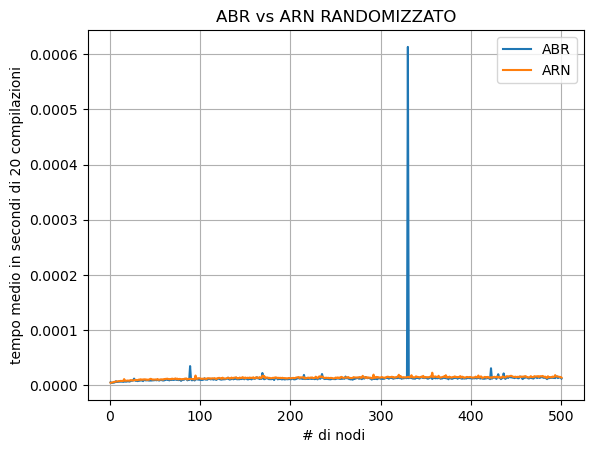
\includegraphics[width = 12cm]{ABR_vs_ARN_RANDOMIZZATO}
\centering
\caption{ABR vs ARN con dimensione crescente e chiavi random}
\label{fig:1}
\end{figure}  


\begin{figure}[H]
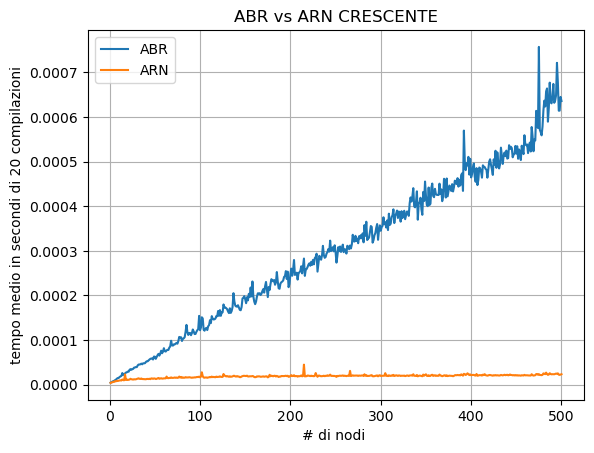
\includegraphics[width = 12cm]{ABR_vs_ARN_CRESCENTE}
\centering
\caption{ABR vs ARN con dimensione crescente e chiavi crescenti}
\label{fig:2}
\end{figure}  

\section{Analisi risultati sperimentali}

\subsection{ABR vs ARN randomizzati}

Come si può notare dalla Figura \ref{fig:1}, l'andamento al crescere della dimensione è quello aspettato.\\
La ricerca in ABR è $O(h)$ dove h è l'altezza dell'albero, che nel caso random è $lg n$.\\
La ricerca in ARN è $O(lg n)$.
Siccome stiamo scorrendo tutti i possibili casi poiché si svolgono ricerche di elementi non appartenenti agli alberi, il tempo è esattamente $lg n$.
Quindi per via sperimentale ci aspettiamo che i tempi di ricerca abbiano all'incirca lo stesso andamento.
Questo fatto avviene, dal grafico possiamo dedurre l'andamento logaritmico del grafico.


\subsection{ABR vs ARN: con inserimento di nodi con chiavi crescenti}

Come si può notare dala Figura \ref{fig:2} l'andamento al crescere della dimensione è quello aspettato.\\
La ricerca in ABR è $O(h)$ dove h è l'altezza dell'albero, in questo caso h = n..\\
La ricerca in ARN è $O(lg n)$.\\
Ci aspettiamo quindi che i tempi di ricerca abbiano un andamento molto diverso: uno lineare, uno logaritmico.
Questo perché ci siamo posti nel caso peggiore, in cui l'algoritmo di ricerca scorre tutti i nodi presenti nel cammino dalla radice alla foglia con la chiave più grande.
Come previsto, l'ABR risulta più lento per via della sua degenerazione in una lista.L'ARN mantiene come previsto un un andamento logaritmico per la ricerca di un elemento anche in questo caso. 

\section{Conclusione}
Come visto dagli esperimenti l’albero rosso nero risulta una struttura più adatta a svolgere ricerche all’interno di essa, grazie al suo bilanciamento dato dal fix-up al momento dell’inserimento di un nuovo elemento.
\end{document}